\documentclass[10pt,a4paper]{article}
\usepackage[utf8]{inputenc}
\usepackage[english]{babel}
\usepackage[T1]{fontenc}
\usepackage{amsmath}
\usepackage{amsfonts}
\usepackage{amssymb}
\usepackage{subcaption}
\usepackage{makeidx}
\usepackage{graphicx}
\usepackage{fourier}
\usepackage{listings}
\usepackage{color}
\usepackage{hyperref}
\usepackage[left=2cm,right=2cm,top=2cm,bottom=2cm]{geometry}
\author{Johannes Scheller (candidate no. 71), Vincent Noculak (candidate no. 22)\\ Lukas Powalla (candidate no. 67), Richard Asbah (candidate no. 50) }
\title{Computational Physics - Project 5}

\lstset{language=C++,
	keywordstyle=\bfseries\color{blue},
	commentstyle=\itshape\color{red},
	stringstyle=\color{green},
	identifierstyle=\bfseries,
	frame=single}
\begin{document}

\maketitle
\newpage
\tableofcontents
\newpage

\begin{abstract}
This report by Richard Absah, Vincent Noculak, Lukas Powalla and Johannes Scheller for the course "FYS3150/4150 - Computational Physics" at the Universitetet i Oslo deals with the computational simulation of a galaxy model. It contains different approaches on solving the differential equations resulting from Newton's law of universal gravitation for objects (e.g. stars) in space. The authors will introduce two algorithms, Velocity Verlet and Runge-Kutta, to solve these differential equations and show both of them in use. They will compare their advantages and disadvantages and finally justify their choice of using Velocity Verlet to simulate n-body system like galaxies. These simulations are used to obtain knowledge about the behaviour of large particle clusters in space, esp. about the collapses these structures perform. Moreover, the authors try to prove powerful statements like the virial theorem by their simulations. The paper ends with an discussion about the future use of the methods use, but also about the problems that occurred during the project. Thus, it will give a small outlook on the limits of the algorithms for future use.
\end{abstract}
\section{Introduction}
When people observe stellar objects like stars or even bigger structures, i.e. galaxies or clusters of galaxies, they soon run into trouble. Despite the fact that many observations by telescopes - no matter with which wavelength they operate - have a very limited accuracy, it is just not possible to obtain precise knowledge about the long term evolution of the motions of these objects and structures in a single lifetime. Even if the first humans had started with exact observations of all the objects they could see, the data collected by theme would be young compared to the lifespan of a galaxy!

On the other hand, we have not found yet analytical solutions for the movements of more than two interacting bodies apart from some special cases with three bodies. As a result of this dilemma - we cannot observe the long-term motion of large stellar systems, but we cannot solve describe them analytically either -, we have to focus on computational simulations of these problems. This is what we are going to try in this project.

In particular, we are going to simulate first two body systems and later on open clusters using Newton's law of universal gravitation. We are going to look at the time an open cluster with a cold collapse would need to collapse into singularity and observe the energy conservation and distribution of potential and kinetic energy. On what properties does it depend how many particles get ejected from the cluster and how do those particles change the energy of the system? The equilibrium state and its radial partial density are going to be observed too.

We are doing these simulations by using both the Velocity Verlet algorithm and the fourth order Runge-Kutta method. First, we are going to compare both algorithms by simulating a to body system. Then we are going to study which algorithm is more suitable for simulating open clusters and continue with these simulations using the algorithm that turned out to be better.
\section{Theory}

\subsection{Newton's law of universal gravitation}

Newton's law of universal gravitation states that every point mass attracts every single other point mass by a force pointing along the line intersecting both points. The force two points of mass with the masses $m_i$ and $m_j$ and a distance of $r_{ij}$ to each other attract each other is given by

\begin{equation}	
\label{eq:gra}
\mathbf{F_G} = - G \frac{m_i \cdot m_j}{r_{ij}^3} \cdot \mathbf{r_{ij}}
\end{equation}

Where $G$ is the gravitational constant. In our project we have a system with $n$ stars which get approximated as points of mass. Hence, to get the gravitational force acting on one star, we just need to sum over all $\mathbf{F}_G$'s (having the form of equation \eqref{eq:gra}) that are acting on this star due to the other stars.

\begin{equation}	
\label{eq:gra2}
\mathbf{F}_{Gi} = \sum_{j \neq i}^{n} - G \frac{m_i \cdot m_j}{r_{ij}^3} \cdot \mathbf{r}_{ij} = - G m_i \sum_{j \neq i}^{n} m_j \frac{\mathbf{r}_{ij}}{r_{ij}^3}
\end{equation}

Then the acceleration of star $i$ is given by

\begin{equation}	
\label{eq:gra3}
\mathbf{a} = - G \sum_{j \neq i}^{n} m_j \frac{\mathbf{r}_{ij}}{r_{ij}^3}
\end{equation}

\subsection{Energy}

In the project we are going to observe the kinetic and potential energy of systems of particles, which interact via the gravitational force. The kinetic energy of a particle with mass $m$ and velocity $v$ is given by $E_{Kin} = \frac{1}{2} m v^2$. Because we have $n$ particles we just need to sum over the kinetic energies of all particles to get the kinetic energy of the system.

\begin{equation}	
\label{en1}
E_{Kin} = \sum_{i = 1}^{n} \frac{1}{2} m_i v_i^2
\end{equation}

The potential energy of a system is given by $\mathbf{\nabla} E_{Pot} = - \mathbf{F}$. Hence we have $\frac{\partial}{\partial x_i}E_{Pot} =- F_{x_i}$ and can get a potential energy by trough integration:

\begin{equation}
\label{en2}
	E_{Pot} = - \int dx' F_{x}(x', y ,z)
\end{equation}

To get the potential energy of our system, we add one particle after an other from an infinite distance to the system. Each time we add a particle $i$ we calculate its potential energy $V_i$ (negative work that is needed to move the particle from an infinite distance to the system) using \eqref{en2}. We do this until we have $n$ particles in the system. Then the potential energy of our system is given by the sum over all $V_i$. If we add the particle 1 there is no force yet, hence $V_1 = 0$. When adding the second particle there is a force between particle 1 and 2. Adding the particle number $i$, there are $i-1$ forces acting on particle $i$(we write the force between particle $i$ and $j$, acting on $i$, as $F_{ij}$). Hence $V_i$ can simply be calculated by

\begin{equation}
\label{en3}
	V_i = - \int_{x_i}^{\infty} dx \sum_{j \neq i}^{i} F_{ij_x}
\end{equation}

And we get

\begin{equation}
\label{en4}
	V_{System} = \sum_{i = 1}^{n} V_i = - \sum_{i = 1}^{n} \int_{x_i}^{\infty} dx \sum_{j \neq i}^{i} F_{ij_x} = - \frac{1}{2} \sum_{i,j = 1; i \neq j}^{n} \int_{x_i}^{\infty} dx F_{ij_x}
\end{equation}

With \eqref{eq:gra} we know

\begin{equation}
\label{en5}
	\int_{x_i}^{\infty} dx F_{ij_x} = - \int_{x_i}^{\infty} dx  G m_i m_j\frac{(x - x_j)}{((x - x_j)^2 + (y_i - y_j)^2 + (z_i - z_j)^2)^\frac{3}{2}} = - \left[ G \frac{m_i m_j}{((x - x_j)^2 + (y_i - y_j)^2 + (z_i - z_j)^2)^\frac{1}{2}}\right]^\infty_{x_i} = G \frac{m_i m_j}{r_{ij}}
\end{equation}

Setting \eqref{en5} in \eqref{en4} we get the potential energy of our system, which is

\begin{equation}
	\label{en6}
	V_{System} = - \frac{1}{2} \sum_{i,j = 1; i \neq j}^{n} G \frac{m_i m_j}{r_{ij}}
\end{equation}

\subsection{Open Clusters}

Open clusters are groups of a few thousand stars that were formed from the same giant molecular cloud and have roughly the same age. They have yet only been found in spiral and irregular galaxies, in which active star formation is occurring.
Many open clusters are unstable and have a small enough mass that the escape velocity of the system is lower than the average velocity of the constituent stars. These clusters will rapidly disperse within a few million years \cite{Link1}

The open cluster we simulate in this project will have the starting conditions of a cold collapse. This means, that the particles start with little or no initial velocity. In addition to the that, the $N$ particles, we simulate, will be randomly uniformly distributed at the starting time inside a sphere with given radius $R_0$. Our particles masses will be distributed by a Gaussian distribution around ten solar masses with a standard deviation of one solar mass.

%If the number of particles goes against infinity ($N \to \infty$), the system should collapse into singularity after a time %$\tau_{crunch} = \sqrt{\frac{3\pi}{32 G \rho_0}}$

\subsection{Verlet algorithm}

The Verlet algorithm is one method that is important to numerically solve a equation of motion having for example the form of equation \eqref{eq:gra2}. 

Using a taylor expansion for a function $x(t)$ around the point $t_0 = t_i$ and then setting $t = t_i + h$ and $t = t_i - h$, we get the equations

\begin{equation}
\label{v1}
x(t_i + h) = x_i + h  x^{'}(t_i) + \frac{h^2}{2}  x^{''}(t_i) + \frac{h^3}{3!}  x^{'''}(t_i) + \sigma (h^4)
\end{equation}
\begin{equation}
\label{v2}
x(t_i - h) = x_i - h  x^{'}(t_i) + \frac{h^2}{2}  x^{''}(t_i) - \frac{h^3}{3!}  x^{'''}(t_i) + \sigma (h^4)
\end{equation}

For an easier overview it is useful to use the notation $x(t_i) = x_i$, $x(t_i \pm h) = x_{i \pm 1}$ and $x^{''} = a(x, t)$. By adding up equation \eqref{v1} and \eqref{v2} we get the equation

\begin{equation}
\label{v3}
	x_{i+1} = 2 x_i - x_{i-1} + a(x_i, t_i) \cdot h^2 + \sigma(h^4)
\end{equation}

Which gives us a method to determine all $x_i$, if the boundary conditions are known. It can be seen that due to the $x_{i-1}$ part in \eqref{v3}, the algorithm is not self-starting. Hence $x_1$ must be found, using an other method (for example Euler's method).

\subsubsection{Velocity Verlet algorithm}

The Velocity Verlet is similar to the Verlet algorithm and is also using Taylor expansions. It uses a half-step velocity $v_{i+\frac{1}{2}}$($v(t) = \frac{dx}{dt}$) to calculate $x_{i+1}$. The first step of the algorithm is to calculate $v_{\frac{1}{2}}$ with \eqref{vv3}, using given $v_0$ and $a(x_0, t_0)$.

\begin{equation}
	\label{vv3}
	v_{i + \frac{1}{2}} = v_i + \frac{h}{2} a(x_i, t_i)
\end{equation}

After this, the algorithm can be executed by simply repeating the following three steps for all $i$.

1.: Calculate
\begin{equation}
	\label{vv4}
	x_{i+1} = x_i +h v_{i+ \frac{1}{2}}
\end{equation}

2.: Calculate $a_{i+1}$ using $x_{i+1}$

3.: Calculate
\begin{equation}
	\label{vv5}
v_{i+\frac{3}{2}} = v_{i+\frac{1}{2}} +h a_{i+1}
\end{equation}

Because we have to calculate $v_\frac{1}{2}$ first, the algorithm is not self-starting. It has to be mentioned, that it is also possible to eliminate the half-step velocities by setting \eqref{vv3} in \eqref{vv4} and \eqref{vv5}. Then, we are using \eqref{vv5} to calculate $v_{i+1}$, by just using the factor $\frac{h}{2}$ instead of $h$ in the formula.
Doing this, we get the formulas

\begin{equation}
\label{vv1}
x_{i+1} = x_i + h \cdot v_i + \frac{h^2}{2}  a_i(x_i, t_i)
\end{equation}

and

\begin{equation}
\label{vv2}
v_{i+1} = v_i + \frac{h}{2} \cdot (a(x_i, t_i) + a(x_{i+1}, t_{i+1}))
\end{equation}

We see, that \eqref{vv2} uses the Trapezoidal rule.
This form of the algorithm starts with calculating equation \eqref{vv1} for $i = 0$ to get $x_{i+1}$. Knowing this value, $a(x_i, t_i)$ and $a(x_{i+1}, t_{i+1})$ can be calculated. Then it is possible to calculate $v_{i+1}$ with equation \eqref{vv2}. These steps can now be repeated for $i = i+1$, allowing to get the values for all $x_i$ and $v_i$.

\subsection{Runge-Kutta methods}

Runge-Kutta methods use the following basic equation of integration to numerically approximate Ordinary differential equations.

\begin{equation}
\label{rc1}
x_{i+1} = x_i + \int_{t_i}^{t_{i+1}} dt^{'} v(x, t^{'})
\end{equation}

With $x(t_i) = x_i$, $x(t_i \pm h) = x_{i \pm 1}$ and $\frac{dx}{dt} = v$. The integral can be approximated using numerically integration methods, as for example the trapezoidal rule or Simpson's rule. In Runge-Kutta methods to calculate a step $x_{i+1}$, an intermediate step between $x_i$ and $x_{i+1}$ gets used.

\subsubsection{fourth order Runge-Kutta method (RK4)}
\label{subsubsec:rc4}

In this project we are going to use the fourth order Runge-Kutta method. This method solves the integral in equation \eqref{rc1} with help of simpson's method. By applying this method we get

\begin{equation}
\label{rc2}
\int_{t_i}^{t_{i+1}} dt^{'} v(t^{'}, x) = \frac{h}{6} [v(t_i, x_i) +4 v(t_{i+\frac{1}{2}}, x_{i+\frac{1}{2}}) + v(t_{i+1}, x_{i+1})] + \sigma(h^5)
\end{equation}

By setting \eqref{rc2} in \eqref{rc1}:

\begin{equation}
\label{rc3}
x_{i+1} = x_i + \frac{h}{6} [v(t_i, x_i) + 2 v(t_{i+\frac{1}{2}}, x_{i+\frac{1}{2}}) + 2 v(t_{i+\frac{1}{2}}, x_{i+\frac{1}{2}}) + v(t_{i+1}, x_{i+1})] + \sigma(h^5)
\end{equation}

$x_{i+\frac{1}{2}}$ and $x_{i+1}$ are unknown values. Now we define $k_1 = v(t_i, x_i)$, first approximate $x_{i+\frac{1}{2}}$ with Euler's method

\begin{equation}
\label{s:rc4}
x_{i+\frac{1}{2}} \approx x_i + \frac{h}{2} v(t_i, x_i) = x_i + \frac{h}{2} k_1
\end{equation}

and define

\begin{equation}
\label{rc5}
k_2 = v(t_{i+\frac{1}{2}}, x_i + \frac{h}{2} k_1)
\end{equation}

Next we calculate $x_{i + \frac{1}{2}}$ with Eulers's method using $k_2$ instead of $k_1$ and then define

\begin{equation}
\label{rc6}
k_3 =  v(t_{i+\frac{1}{2}}, x_i+\frac{h}{2} k_2)
\end{equation}

We predict $x_{i+1}$ with $k_3$ using Euler's method

\begin{align}
x_{i+1} = x_i + h k_3 \\
k_4 = v(t_{i+1}, x_i + h k_3)
\end{align}

Now we can calculate our final $x_{i+1}$ by inserting our $k_j$'s in equation \eqref{rc3}.

\begin{equation}
\label{rc9}
x_{i+1} =  x_i + \frac{h}{6} (k_1 + 2 k_2 + 2 k_3 + k_4) + \sigma(h^5)
\end{equation}

\subsubsection{RK4 in this Project}

In section \ref{subsubsec:rc4} it could be seen, that with the fourth order Runge-Kutta method, first-order ODE's (ordinary differential equations) can be solved. In this project however, we need to numerically solve the equation of motion for multiple particles, which is a second-order ODE (see equation \eqref{eq:gra3}). This ODE can be split up into two first-order ODE's by writing

\begin{align}
\frac{d\mathbf{r}}{dt} = \mathbf{v}  \\
\frac{d\mathbf{v}}{dt} = G \sum_{j \neq i}^{n} m_j \frac{\mathbf{r}_{ij}}{r_{ij}^3}
\end{align}

Now we can use the RK4 method $\mathbf{r}$ and $\mathbf{v}$ simultaneously. Because we use this method in three dimensions and the fact, that we have a second-order ODE, the equations for the RK4 method look different than in section \ref{subsubsec:rc4}. The following steps give in the right order, how to approach the system, when we do a numerically calculation from the time $t_i$ to $t_{i+1}$. It has to be noted, that when we do a calculation for one particle, directly after it, the same type of calculation gets performed for the other particles. The index on the upper left side of values refer to the number of the particle and the index on the upper right side gives the information, if the value is belogs to the RK4 method for the location or the velocity.

\begin{align}
\label{rc11}
\mathbf{k}_1^r = \mathbf{v}_i \\
\mathbf{k}_{1}^{v} = \mathbf{a}({}^{1}\mathbf{r}_i, {}^{2}\mathbf{r}_i,..., {}^{N}\mathbf{r}_i) \\
\mathbf{k}_2^r = \mathbf{v}_i + \frac{h}{2} \mathbf{k}_1^{v}	\\
\mathbf{k}_2^{v} = \mathbf{a}({}^{1}\mathbf{r}_i + \frac{h}{2}\cdot {}^{1}\mathbf{k}_1^r, {}^{2}\mathbf{r}_i + \frac{h}{2}\cdot {}^{2}\mathbf{k}_1^r,..., {}^{N}\mathbf{r}_i + \frac{h}{2}\cdot {}^{N}\mathbf{k}_1^r)	\\
\mathbf{k}_3^r = \mathbf{v}_i + \frac{h}{2} \mathbf{k}_2^v	\\
\mathbf{k}_3^{v} = \mathbf{a}({}^{1}\mathbf{r}_i + \frac{h}{2}\cdot {}^{1}\mathbf{k}_2^r, {}^{2}\mathbf{r}_i + \frac{h}{2}\cdot {}^{2}\mathbf{k}_2^r,..., {}^{N}\mathbf{r}_i + \frac{h}{2}\cdot {}^{N}\mathbf{k}_2^r)	\\
\mathbf{k}_4^r = \mathbf{v}_i + h \cdot \mathbf{k}_3^v	\\
\label{rc12}
\mathbf{k}_4^{v} = \mathbf{a}({}^{1}\mathbf{r}_i + h\cdot {}^{1}\mathbf{k}_3^r, {}^{2}\mathbf{r}_i + h\cdot {}^{2}\mathbf{k}_3^r,..., {}^{N}\mathbf{r}_i + h\cdot {}^{N}\mathbf{k}_3^r)
\end{align}

The accelerations can always get calculated by using equation \eqref{eq:gra3}. After the steps of equations \eqref{rc11} to \eqref{rc12} are executed, the velocity and positions of the particles for the time $t_{i+1}$ can be calculated using formula \eqref{rc9}.

\section{Execution}

In this project we are programming the motion of a n-body system. We are using two different algorithms for calculating the motion of the bodies called the Velocity-Verlet-algorithm and the Runge-Kutta-algorithm. 
We started to set up an algorithm for a two body system because this is much easier than dealing with n-bodies. However, we think it is sufficient to describe the program for n-bodies because the two body case is there also included. In our case, the bodies are represented by planets. 
\subsection{General structure and overview}
We are using several classes in order to structure our program. The first class is called planet. Objects out of this class represent Planets with properties such as the position, velocity and mass. Originally, we thought that it would be nice to work with the planet objects and its positions and velocities in the algorithms itself. However, the Runge-Kutta method is heavily readable using this representation. Therefore, we used a matrix representation for position and velocity. The important information about position and velocity in kept in the matrix A. 
The second class is called solarsystem. This class contains all important functions and algorithms used to calculate the motion of the system. 
The header file for the basic functions looks as follows: (functions to calculate the Energy of the system (kinetic and potential) and to check the Virial theorem will be explained at a later point)
\begin{lstlisting}
class solarsystem
{
public:
    //constructor
    solarsystem();
    //constants and arrays used for Energy-analysis
    double* vecKinpot;
    double* finalEnergy;
    vector<double> average_kin; 
    vector<double> average_pot; 
    //other constants and objects 
    double R0=20;
    double averagemass=10;
    int numplanets;
    double G;
    double epsilon=0.002;
    vector<Planet> planets;
    Mat<double> A;
    Mat<double> dA;
    // use of the random class
    std::random_device rd;
    std::mt19937 gen;
    std::uniform_real_distribution<> dis;
    gaussian_random object;
    //general functions
    void addplanet(Planet Planet1);
    void addrandomplanet(double R_0);
    void setmatrices();
    //functions used only for Velocity-Verlet
    void VelocityVerlet(double dt,int n);
    void calculateForces();
    //Functions used only for Runge-Kutta-method
    void RungeKuttamethod(double dt,int n);
    mat derivate( Mat<double> B);
     // funktions for Energy-analysis
    void kinPotEnergy();  //VelocityVerlet RK-4
    void virial_output();
};
\end{lstlisting}
We will now briefly explain the use of the constructor, constants and functions of the class solarsystem. The functions, which are specific to Velocity-Verlet or Runge-Kutta method are explained in the section named after the method. The use of the random class itself will not be explained here. We are using a random number generator with a period of $2^{32}$. This is sufficient. The random number generator is seeded by default while constructing a object of solarsystem. 
\subsubsection{constructor}
We need a constructor in order to create objects of the class. With constructing the class, we also initialise the random number generator and set the number of planets of the created solarsystem-object to 0. 
\begin{lstlisting}
solarsystem::solarsystem() : gen(this->rd()), dis(0,1)
{
    this->numplanets=0;
}
\end{lstlisting}
\subsubsection{constants and objects}
We need some constants for the random number generator in order to create random planet-objects with the right properties. R0 is the radius for the sphere in which the planets should be distributed with constant particle density. The average-mass (averagemass) is the averagemass of the random planet-objects. The standard deviation of the planet objects is manually set to a specific value in the function addrandomplanet(double R0). The integer numplanets counts the actual number of planets of a specific planet object. The gravitational constant G is in our case dependent on the number of planets and the average-mass of a planet. Therefore, this constant is recalculated every time you add a planet. (in the function addrandomplanet) 
The smoothing-factor epsilon is also initialised and defined. 
\subsubsection{general functions} 
Our n-body- system can be used in different ways. You can manually add a planet with chosen initial position, initial velocity and mass. This is done by the function addplanet(Planet Planet1). Therefore, this algorithm can also be used to calculate the motion of a given two body system. With small changes, it is also be possible to simulate our solar-system. (G has to be changed)
\begin{lstlisting}
void solarsystem::addplanet(Planet Planet1){
    planets.push_back(Planet1); //  adds the planet to the vector of planets
    average_kin.push_back(0);
    average_pot.push_back(0);
    this->numplanets+=1;
    G=4*M_PI*M_PI*R0*R0*R0/(32*this->numplanets*averagemass);
}
\end{lstlisting}
On the other way, you can choose to add a planet with random position within a sphere and with given Gaussian-distributed mass of the planet. This is done by the function addrandomplanet(double R0 ). We set the planet-velocities to 0. With Box–Muller transform, we get a normal-distribution with given mean-value and given standard-deviation. The mass is set to a random Gaussian-distributed value. We wand a equal density at t=0 within a sphere. Therefore, we have to manipulate a random generated triple (u,v,w between 0 and 1) as follows:
\begin{align*}
r &=R0 \cdot \sqrt[3]{u} \\
\theta &= \arccos(1-2v) \\
\phi &= 2 \pi \omega
\end{align*}
We want to use spherical coordinate. Therefore, we transform back to spherical coordinates, simplify and get:
\begin{align*}
x&=R0 \cdot \sqrt[3]{u} \cdot  \sqrt{1-(1-2\cdot v)^{2} }\cdot cos(2\pi \cdot \omega) \\
y&=R0 \cdot \sqrt[3]{u} \cdot  \sqrt{1-(1-2\cdot v)^{2} }\cdot sin(2\pi \cdot \omega) \\
z &= R0 \cdot \sqrt[3]{u} \cdot (1-2 \cdot \omega )
\end{align*}
In the end, we add the new planet with the function addplanet to the solarsystem. 
\begin{lstlisting}
void solarsystem::addrandomplanet(){
    Planet randomplanet;
    // set andom mass with Gaussian-distribution
    randomplanet.m=object.generateGaussianNoise(10,1);
    // set velocities to 0
    randomplanet.velocity[0]=0;
    randomplanet.velocity[1]=0;
    randomplanet.velocity[2]=0;
    //generate random position
    double r=dis(gen);
    double theta=dis(gen);
    double phi=dis(gen);
    //transform random position in order to get
    //Cartesian coordinates with constant density
    randomplanet.position[0]=R0*pow(r,(1.0/3.0))*sqrt((1-(pow(1-2*theta,2))))*cos(2*M_PI*phi);
    randomplanet.position[1]=R0*pow(r,(1.0/3.0))*sqrt((1-(pow(1-2*theta,2))))*sin(2*M_PI*phi);
    randomplanet.position[2]=R0*pow(r,(1.0/3.0))*(1-(2*theta));
    addplanet(randomplanet);
}
\end{lstlisting}

To use the matrix-representation of position and velocity, we wrote the function setmatrices(), which constructs a martix A, which contains all positions and velocities of the planets, which has been added to the system so far. The position of the planets can be found in the first column and the velocity in the second column. Every planet has 3 Space-Coordinates and 3 Velocity-Coordinates. In addition to that, setmatrices() constructs the matrix dA, which is the time derivative of the matrix A. This means that in the first column are velocities and in the second column are accelerations. For RK4, this is really useful because we can perform very understandable operations like $A=A+dA \cdot dt $.
Notice, that the velocity sits in the second column of A as well as in the first column of dA.
\begin{align}
A=
\begin{bmatrix}
r_{x_1} & v_{x_1}\\
r_{y_1} & v_{y_1} \\
r_{z_1} & v_{z_1} \\
r_{x_2} & v_{x_2} \\
... & ... \\
r_{x_n} & v_{x_n}\\
r_{y_n} & v_{y_n} \\
r_{z_n} & v_{z_n} \\
\end{bmatrix}
& &
dA=
\begin{bmatrix}
v_{x_1} & a_{x_1}\\
v_{y_1} & a_{y_1} \\
v_{z_1} & a_{z_1} \\
v_{x_2} & a_{x_2} \\
... & ... \\
v_{x_n} & a_{x_n}\\
v_{y_n} & a_{y_n} \\
v_{z_n} & a_{z_n} \\
\end{bmatrix}
\end{align}
\begin{lstlisting}
void solarsystem::setmatrices(){
    A=Mat<double>(this->numplanets*3,2);
    dA=Mat<double>(this->numplanets*3,2);
    
    for(int i=0;i<this->numplanets;i+=1){
        for(int j=0;j<3;j++){
            A(3*i+j,0)=planets[i].position[j];
            A(3*i+j,1)=planets[i].velocity[j];
        }
    }
    
    for(int i=0;i<this->numplanets;i+=1){
        for(int j=0;j<3;j++){
            dA(3*i+j,0)=planets[i].velocity[j];
            dA(3*i+j,1)=planets[i].force[j]/planets[i].m;
        }
    }
}
\end{lstlisting}


\subsection{Velocity-verlet-algorithm}
In the following, we find the central steps for implementing the Velocity-verlet-algorithm. This is a non-selfstarting algorithm because we need to calculate v(t+0.5dt) before entering the loop of the algorithm. We are using the velocity in the first column of the matrix A for calculations.  
\begin{lstlisting}
void solarsystem::VelocityVerlet(double dt,int n){
  ...
   setmatrices();
   calculateForces();                              
   A.col(1)=A.col(1)+0.5*dt*dA.col(1); // v(t)->v(t+0.5dt)
   for(int k=0;k<n;k++){
      A.col(0)=A.col(0)+A.col(1)*dt;   // r(t+dt)
      calculateForces();               // a(t+dt)
      A.col(1)=A.col(1)+dt*dA.col(1);  // v(t+0.5dt) -> v(t+3/2dt)
      for(int i=0;i<this->numplanets;i+=1){
      dA.col(0)=A.col(1); //updating velocities in dA, not necessary
        }
      }
  ...
}
\end{lstlisting}
The function calculateForces() calculates the forces of all the planets and with that the acceleration and writes it into the matrix dA. The forces of the planetobjects are primarily used for local calculations. 
\begin{lstlisting}
void solarsystem::calculateForces(){

    
    for(int k=0;k<this->numplanets;k++){
        for(int l=0;l<3;l++){
            planets[k].force[l]=0;
        }
    }
    for(int i=0;i<this->numplanets;i++){
        for(int j=i+1;j<this->numplanets;j++){
            double dx=A(3*i,0)-A(3*j,0);
            double dy=A(3*i+1,0)-A(3*j+1,0);
            double dz=A(3*i+2,0)-A(3*j+2,0);
            double dr2=dx*dx+dy*dy+dz*dz+epsilon*epsilon;
            //calculate forces
            double Fx=(G*(planets[i].m)*(planets[j].m)*dx)/pow(dr2,1.5);
            double Fy=(G*(planets[i].m)*(planets[j].m)*dy)/pow(dr2,1.5);
            double Fz=(G*(planets[i].m)*(planets[j].m)*dz)/pow(dr2,1.5);
            //update planet properties
            planets[i].force[0]-=Fx;
            planets[j].force[0]+=Fx;
            planets[i].force[1]-=Fy;
            planets[j].force[1]+=Fy;
            planets[i].force[2]-=Fz;
            planets[j].force[2]+=Fz;
        }
    }
    //update the matrix dA
    for(int i=0;i<this->numplanets;i+=1){
        for(int j=0;j<3;j++){
            dA(3*i+j,1)=planets[i].force[j]/planets[i].m;
        }
    }
    
}
\end{lstlisting}

\subsection{Runge Kutta-Method}
We use the matrix representation for the RK4-Method. We first calculate the derivatives of the matrix A at different times and store them in the matrices k1 to k4. Afterwards, we simply numerically integrate using the coefficients given by the formula of RK4. In this representation, the algorithm is very compact and easily readable.  
\begin{lstlisting}
void solarsystem::RungeKuttamethod(double dt,int n){
    setmatrices();
    Mat<double> k1,k2,k3,k4;
    k1=Mat<double>(this->numplanets*3,2);
    k2=Mat<double>(this->numplanets*3,2);
    k3=Mat<double>(this->numplanets*3,2);
    k4=Mat<double>(this->numplanets*3,2);

    for(int i=0;i<n;i++){
        k1=derivate(A);
        k2=derivate(A+k1*(dt/2));
        k3=derivate(A+k2*(dt/2));
        k4=derivate(A+k3*dt);
        A=A+(1.0/6.0)*(k1+2*k2+2*k3+k4)*dt;
        }
    }
}
\end{lstlisting}
The function derivate( Mat<double> B) calculates the derivative of the matrix in the argument B. The function uses the positions stored in the matrix B to calculate the forces of the planets. Finally, we can calculate the accelerations on the planets using their mass. We write the velocity of the first column of B into the 0th column of dB and we write the calculated accelerations in the first column of dB. 
In total, we calculated and return the derivative of the input matrix B.
\begin{lstlisting}
mat solarsystem::derivate( Mat<double> B){
    Mat<double> dC;
    dC=Mat<double>(this->numplanets*3,2,fill::zeros);
    for(int i=0;i<this->numplanets;i++){
        for(int j=i+1;j<this->numplanets;j++){
            double dx=B(3*i,0)-B(3*j,0);
            double dy=B(3*i+1,0)-B(3*j+1,0);
            double dz=B(3*i+2,0)-B(3*j+2,0);
            double dr2=dx*dx+dy*dy+dz*dz+epsilon*epsilon;
            //calculate forces
            double Fx=(G*(planets[i].m)*(planets[j].m)*dx)/pow(dr2,1.5);
            double Fy=(G*(planets[i].m)*(planets[j].m)*dy)/pow(dr2,1.5);
            double Fz=(G*(planets[i].m)*(planets[j].m)*dz)/pow(dr2,1.5);
            dC(3*i,1)-=Fx;
            dC(3*j,1)+=Fx;
            dC(3*i+1,1)-=Fy;
            dC(3*j+1,1)+=Fy;
            dC(3*i+2,1)-=Fz;
            dC(3*j+2,1)+=Fz;
        }
    }
    for(int i=0;i<this->numplanets;i+=1){
        for(int j=0;j<3;j++){
            dC(3*i+j,1)=dC(3*i+j,1)/planets[i].m;
        }
    }
    dC.col(0)=B.col(1);
    return(dC);//return dC with velocity from B and new acceleration
}
\end{lstlisting}
\subsection{Additional methods}
In order to analyse our data we need to find the potential energy and the kinetic energy at a given time $t$. Down here is the void function \emph{KinpotEnergy} which calculates both the kinetic and potential energy for each particle. When ever this function is called in our RK4 or verlet method it calculates these values for one time step.
\begin{lstlisting}
kineticEnergy <vector> //where we store each particle kinetic energy 
potentialEnergy <vector> //where we store each particle potential energy 

theTotalEnergy // where we store the total energy for all particles
total_kin // where we store the total kinetic energy only for the particles in system
total_pot // where we store the total potential energy only for the particles in system
numplanetsInSystem // the number of particles still in the system
ergodic //the value of ergodic ratio 
\end{lstlisting}

\begin{lstlisting}
void solarsystem::kinPotEnergy(){

kineticEnergy = new double[ this->numplanets];
total_kin = 0.0;
total_pot = 0.0;

double potenial = 0.0;
double totalKinetic = 0.0;
double totalPotenial = 0.0;
double velocitySquared= 0.0;

//kineticEnergy = 1/2 * m * v^2
for (int i = 0; i < this->numplanets;i++){
velocitySquared = A(3*i,1)*A(3*i,1)+A(3*i+1,1)*A(3*i+1,1)+A(3*i+2,1)*A(3*i+2,1);
kineticEnergy[i] = 0.5*planets[i].m*velocitySquared;

totalKinetic += kineticEnergy[i];
}

//potineal energy U = -G Mm/r----------------
potentialEnergy = new double[ this->numplanets];
double r;
Mat<double> p = Mat<double>(this->numplanets,this->numplanets,fill::zeros); //matrix p will include the potenail form all planets.

for (int i = 0;i < this->numplanets; i++ ){
for (int j = i+1; j < this->numplanets; j++){
r = (A(3*i,0)- A(3*j,0))*(A(3*i,0)- A(3*j,0)) + (A(3*i+1,0)- A(3*j+1,0))*(A(3*i+1,0)- A(3*j+1,0))+(A(3*i+2,0)- A(3*j+2,0))*(A(3*i+2,0)- A(3*j+2,0));
r = sqrt(r);
p(i,j)=-planets[i].m*planets[j].m*G/r;
p(j,i)=p(i,j);
totalPotenial += p(j,i);
}
}
//calcuting the potenial energy for each planet from the marix P
for(int i = 0; i < this->numplanets; i++){
for(int j = 0; j < this->numplanets; j++){
potenial += p(i,j);
}
potentialEnergy[i] = potenial;
potenial = 0;
}
theTotalEnergy = totalKinetic+totalPotenial;

//Virial analysis
numplanetsInSystem = 0;

//clac the energy of the bound system ! virial !!!
for (int i = 0;i < this->numplanets; i++ ){
if (( kineticEnergy[i]+potentialEnergy[i])<0.0){
numplanetsInSystem += 1;
total_kin += kineticEnergy[i];
total_pot += potentialEnergy[i];
}

}
total_pot = total_pot/2;
ergodic = total_pot/total_kin;
}
\end{lstlisting}
In the first part of the function, we calculate the kinetic energy for each particle as $1 \frac{1}{2}m v(t)^2 $

In the second part, we calculate all the potentials between different particles in a matrix p in the following way:

\begin{align}
p=
\begin{bmatrix}
0 & \frac{-Gm_1m_0}{r} & \frac{-Gm_2m_0}{r} & ... & \frac{-Gm_nm_0}{r}  \\
\frac{-Gm_0m_1}{r} & 0 & \frac{-Gm_2m_1}{r} & ... & \frac{-Gm_nm_1}{r}  \\
... & ... & ... & ... & ... \\
\frac{-Gm_0m_n}{r} & \frac{-Gm_1m_n}{r} & \frac{-Gm_2m_n}{r} & ... & 0  \\
\end{bmatrix}
\end{align} 
Afterwards, we perform a new for loop, where we calculate the potential energy for a particle $i$ as the sum over al elements of the $i$th row, and finally calculate the total potential and kinetic of the system by summing only over the bounded particle by using an if test to get only the particles with negative total energy.

In the method \emph{centermassfunction}, we calculate the centre of mass $\mathbf{r}_c$ of the system. We loop over all bounded particles $\mathbf{r}_c = \frac{\sum\limits_{i=1}^n m_i*\mathbf{r}_i}{m_\mathrm{total}}$
\begin{lstlisting} 
void solarsystem::centermassfunction(){
centermass = new double[3];//(centrMassX,centerMassY,centerMassZ)
double centermassX = 0.0;
double centermassY = 0.0;
double centermassZ = 0.0;
double totalmass = 0.0;
for (int i = 0;i<this->numplanets;i++){
if (( kineticEnergy[i]+potentialEnergy[i])<0.0){
totalmass  += planets[i].m;
centermassX += A(3*i,0)*planets[i].m;
centermassY += A(3*i+1,0)*planets[i].m;
centermassZ += A(3*i+2,0)*planets[i].m;
}
}
centermassX = centermassX/totalmass;
centermassY = centermassY/totalmass;
centermassZ = centermassZ/totalmass;
centermass[0] = centermassX;
centermass[1] = centermassY;
centermass[2] = centermassZ;
}
\end{lstlisting}
\clearpage
\section{Results}

\subsection{Results of the two-body-system}

We first test our two body algorithm with well known systems in order to check whether we can reproduce our predictions. We simulate the earth and the sun. With Velocity Verlet algorithm, we get figure \ref{TWOB_earth-sun-Verlet} and with the forth order Runge Kutta method (RK4), we get figure \ref{TWOB_earth-sun-RK4}. Both trajectories fit to what we expect from the system. We see a circular motion. We can't see a qualitative difference of the two calculated trajectories. 
Next, we test our two-body solver with a bit more complicated initial conditions. The initial conditions can be looked up in the figures itself. We get for Verlet the figure \ref{TWOB_Verlet_example} and for RK4 the figure \ref{TWOB_RK4_example}. We get the qualitative correct movement of both planets and we can't see qualitative differences of the two solvers. 


\begin{figure}[h]
\centering
\begin{subfigure}{0.45\textwidth}
\centering
	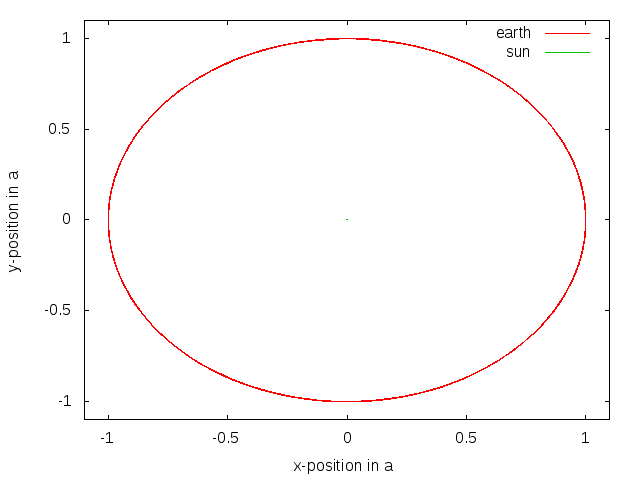
\includegraphics[width=\textwidth]{Verletposition_sun_earth.png}
	\caption{sun-earth system simulated for 10y with Verlet-method\label{TWOB_earth-sun-Verlet}}
\end{subfigure}
\begin{subfigure}{0.45\textwidth}
\centering
	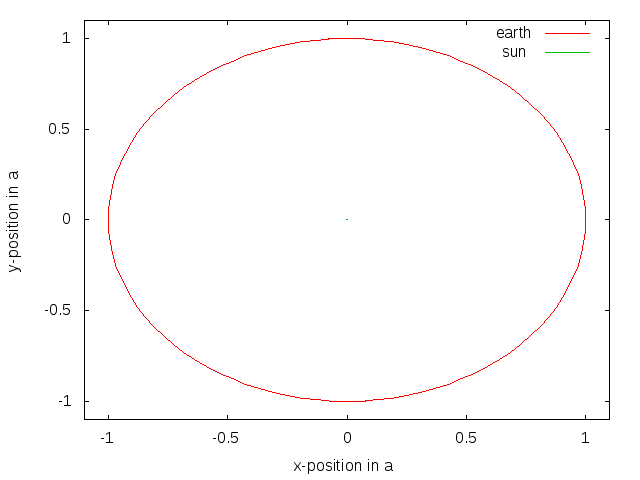
\includegraphics[width=\textwidth]{Rungekuttaposition_sun_earth.png}
	\caption{sun-earth-system simulated for 10y with RK4-method \label{TWOB_earth-sun-RK4}}
\end{subfigure}
\begin{subfigure}{0.45\textwidth}
\centering
	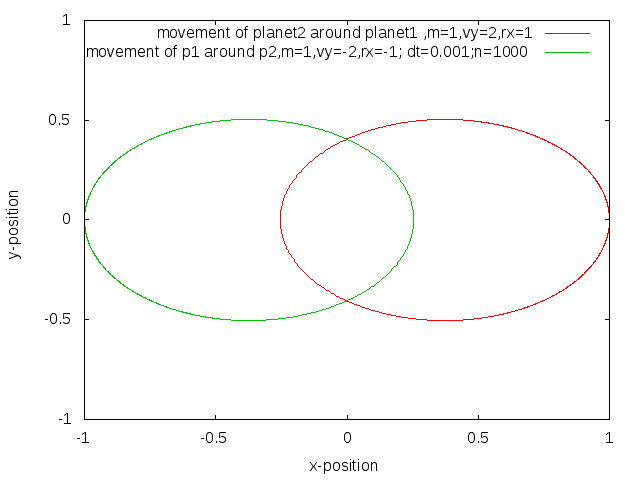
\includegraphics[width=\textwidth]{Verletposition_two_planets.png}
	\caption{two-body-problem solved with Verlet\label{TWOB_Verlet_example}}
\end{subfigure}
\begin{subfigure}{0.45\textwidth}
\centering
	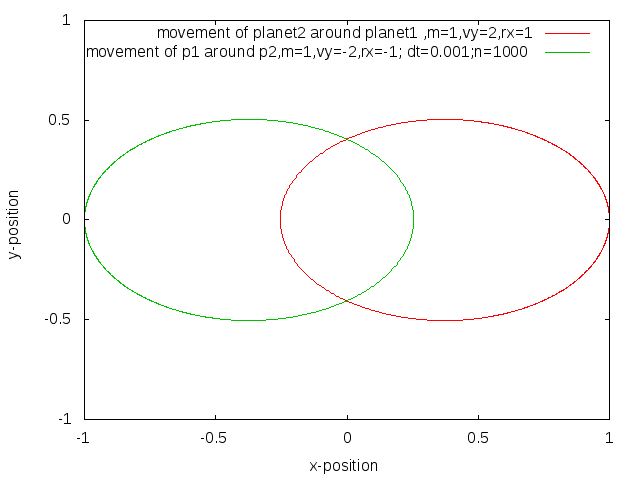
\includegraphics[width=\textwidth]{Rungekuttaposition_with_lines.png}
	\caption{two-body-problem solved with RK4 \label{TWOB_RK4_example}}
\end{subfigure}
\caption{two-body-problem-plots}
\end{figure} 

Since we use two different solvers, we want to know how they differ with respect to large time-steps and long times in order to say which of them should be used for which case. For fairly large time-steps, we clearly saw the difference. With time-steps of 35.6 days the Verlet-algorithm in figure \ref{TWOB_earth-sun-Verlet-largetimesteps} is more stable than the RK4-algorithm in figure \ref{TWOB_earth-sun-RK4-largetimesteps}. Using RK4, the earth is in the end not bound any more. For large time-steps it seems therefore to be better to use Verlet-algorithm. 

\begin{figure}[h]
\centering
\begin{subfigure}{0.45\textwidth}
\centering
	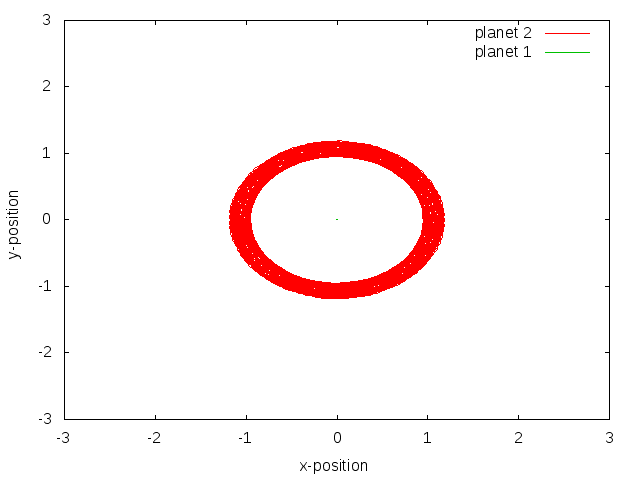
\includegraphics[width=\textwidth]{Verletposition2largetimesteps.png}
	\caption{sun-earth system simulated with Verlet-method; positions in earth-sun-distances \label{TWOB_earth-sun-Verlet-largetimesteps}}
\end{subfigure}
\begin{subfigure}{0.45\textwidth}
\centering
	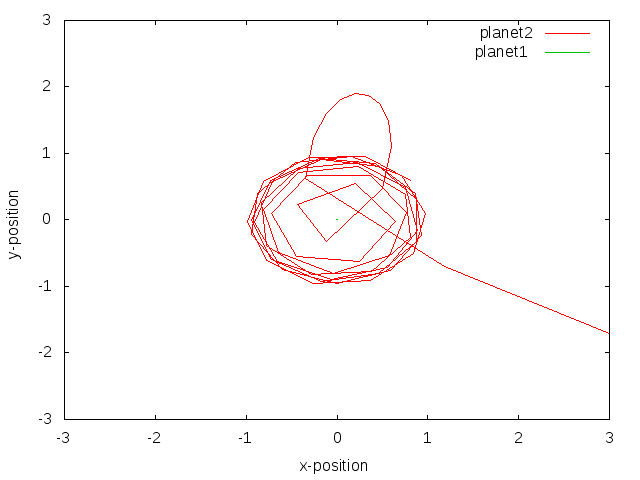
\includegraphics[width=\textwidth]{Rungekuttaposition_largetimesteps.png}
	\caption{sun-earth-system simulated with RK4-method; positions in earth-sun-distances \label{TWOB_earth-sun-RK4-largetimesteps}}
\end{subfigure}
\caption{analysis of large time-steps for the two-body-problem of the sun (planet1) and the earth (planet2) for dt=0.1 and n=1000; This is equivalent to 100 years with time-steps of approximately 36.5 days }
\end{figure}

However, it was hard to find out a difference of the two solvers for very long times. It seemed to be as if they were both accurate. We decided to look at the Energy-conservation of the two systems. We simulates 10000 years (dt=0.001 n=10000000 ) with both methods. The Verlet-algorithm was much faster than the RK4-algorithm. This will be important when we decide which we use for the n-body-problem. 
The plot of the trajectories of both methods look qualitatively good. That means that both algorithms are stable. In both methods, the earth orbits the sun in a stable orbit. 
In order to say something about the accuracy of the algorithms, we looked at the total energy of the system. We calculated the quotient of the total energy of the system at the end of the calculations and the total energy of the system at the beginning of the calculations. (a corresponds to 1 year and au to 1 astronomical unit) We found out that for large times, RK4-algoritm is a bit more precise than the Verlet-algorithm. However, RK4 is numerically much more expensive.(comparing FLOPS and computation time) (see table \ref{TWOB_Energy_analysis} for Energy analysis) 
\begin{table}[h]
\centering
\caption{Analysis of energy conservation of Verlet/RK4-algorithm for dt=0.01 and n=10000000. This corresponds to 10000 years. We are comparing the total energy in the beginning wit the total energy in the end. Before doing that, we convinced ourselves that both methods are stable \label{TWOB_Energy_analysis}}
\begin{tabular}{c|c|c}
&Verlet & RK4 \\
\hline \hline
$E_{tot,i}$in $\frac{M_o au^2}{a^2}$ &5.92174 $10^{-5}$ &5.92174 $10^{-5}$ \\
$E_{tot,f}$in $\frac{M_o au^2}{a^2}$ &5.91593 $10^{-5}$ &5.92173 $10^{-5}$ \\
\hline
$\frac{E_{tot,f}}{E_{tot,i}}$ & 0.99902& 0.99999\\
\end{tabular}
\end{table}

\subsubsection{Conclusion of the results of the two-body-system}

We recommend for large time-steps the Verlet-algorithm because the trajectory calculated with Verlet was more stable than the trajectory calculated with RK4-method. 
For long times, we found out that the RK4-algorithm is a bit more accurate than the Verlet-algorithm. We derived this result from looking at the energy conservation. However, the RK4-algorithm is numerically more expensive than the Verlet-algorithm. Therefore, it could also make sense to run programs with higher numbers of n with the Verlet-algorithm.

\subsection{$N$-body system}
In fig. \ref{c1}, we plotted the development of the total energy over time in units of the initial total energy $E_0$. It has to be noted that this initial energy has a negative value as it only consists of potential energy! We can see that we get more and more kinetic energy in our system, slowly reaching a positive total energy at $t_\mathrm{crunch}$. Shortly after that, we reach a stable state for our system with $E=-4E_0$.

The particles that get ejected from our system are obviously unbound. That means that the absolute value of the kinetic energy of these unbound particles is higher than the absolute value of the potential energy. As the potential energy has a negative sign, this is equivalent to positive total energy! This makes it very easy to identify the particles that got ejected and aren't in our system any more: We just look for the objects with a positive total energy. The fraction of such particles on the total number of objects in the system is plotted in fig. \ref{d2} as a function of time for three different total numbers of particles in the system. We can see that this percentage obviously increases with time for all sizes of the system until it more or less reaches a stable state. This is obvious as in the beginning where all particles are at rest, none of them can have kinetic energy that is higher than the potential energy, so the first particles get ejected after some time. Just when the system begins to reach a more or less stable state, the crunch sets in. As the objects get very close in this event, many of them get accelerated very fast and the number of unbound particles increases again. An interesting thing that can be observed is that for a higher number of particles in total, the share of unbound ones will set at a higher value! Our explanation for this effect is that if our total number of particles is higher for the same radius of our system, the density of particles is obviously higher. This implies that there is a higher probability of particles 'hitting' each other and therefore getting accelerated very fast.

In fig. \ref{d3}, we can see what the ejection of particles means for the total energy. This plot shows the total energy of the system (again in units of $E_0$) against the number of particles that are not ejected from he system. Every data point in this diagram shows the number of bound particles and the corresponding energy after a time step. We know from the last digram, that the number of bound particles slowly decreases over time. This diagram shows that every time an object gets ejected, the total energy gets closer to $0$, meaning that we lose potential energy and gain kinetic energy. This sounds reasonable as an ejected planet has a high velocity (meaning high kinetic energy), but will soon have a large distance to the remaining system, leading to a very small contribution to the total potential energy.
\begin{figure}[h]
	\caption{The total energy of the system over time, without smoothing 		function\label{c1}}
	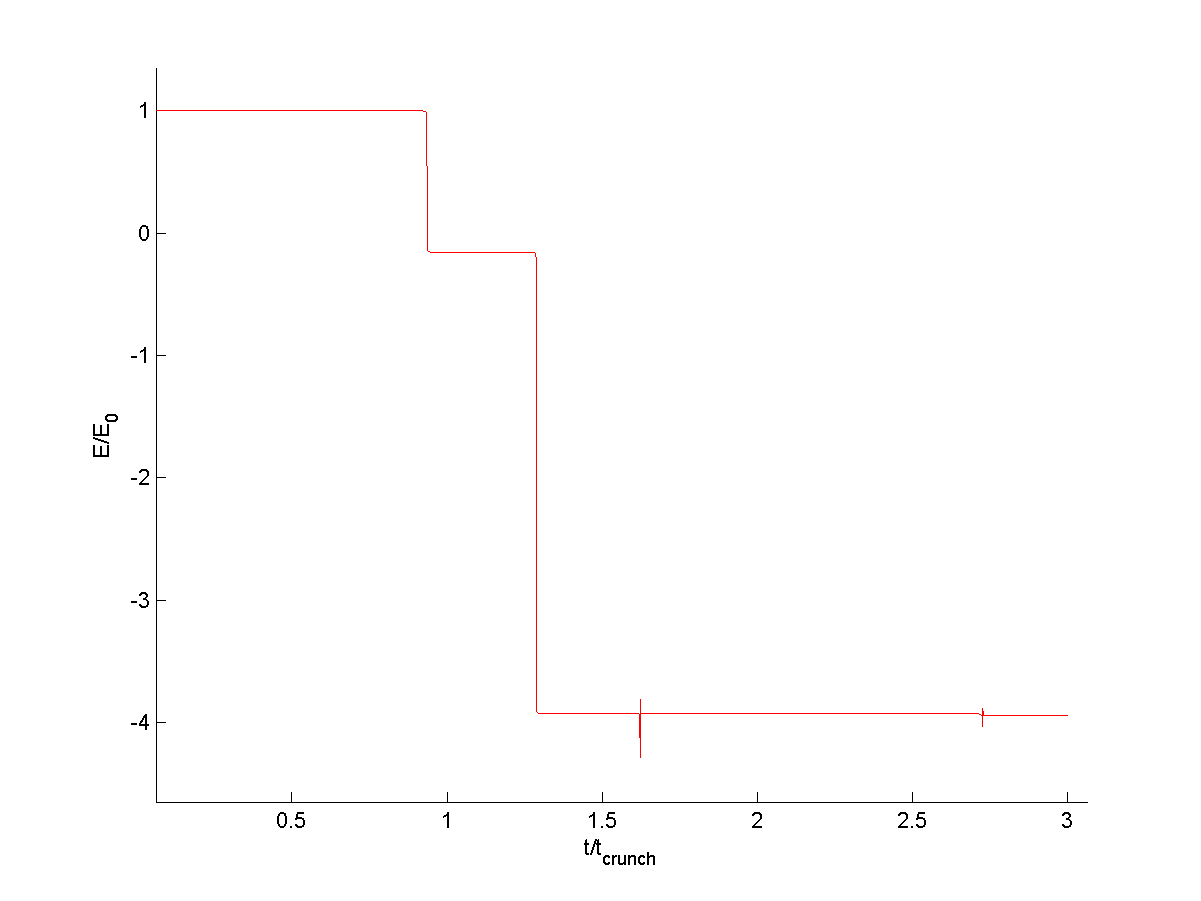
\includegraphics[width=0.8\textwidth]{c1.png}
\end{figure}
\begin{figure}[h]
	\caption{The fraction of particles with positive energy (=ejected particles) as a function of time, without smoothing factor\label{d2}}
	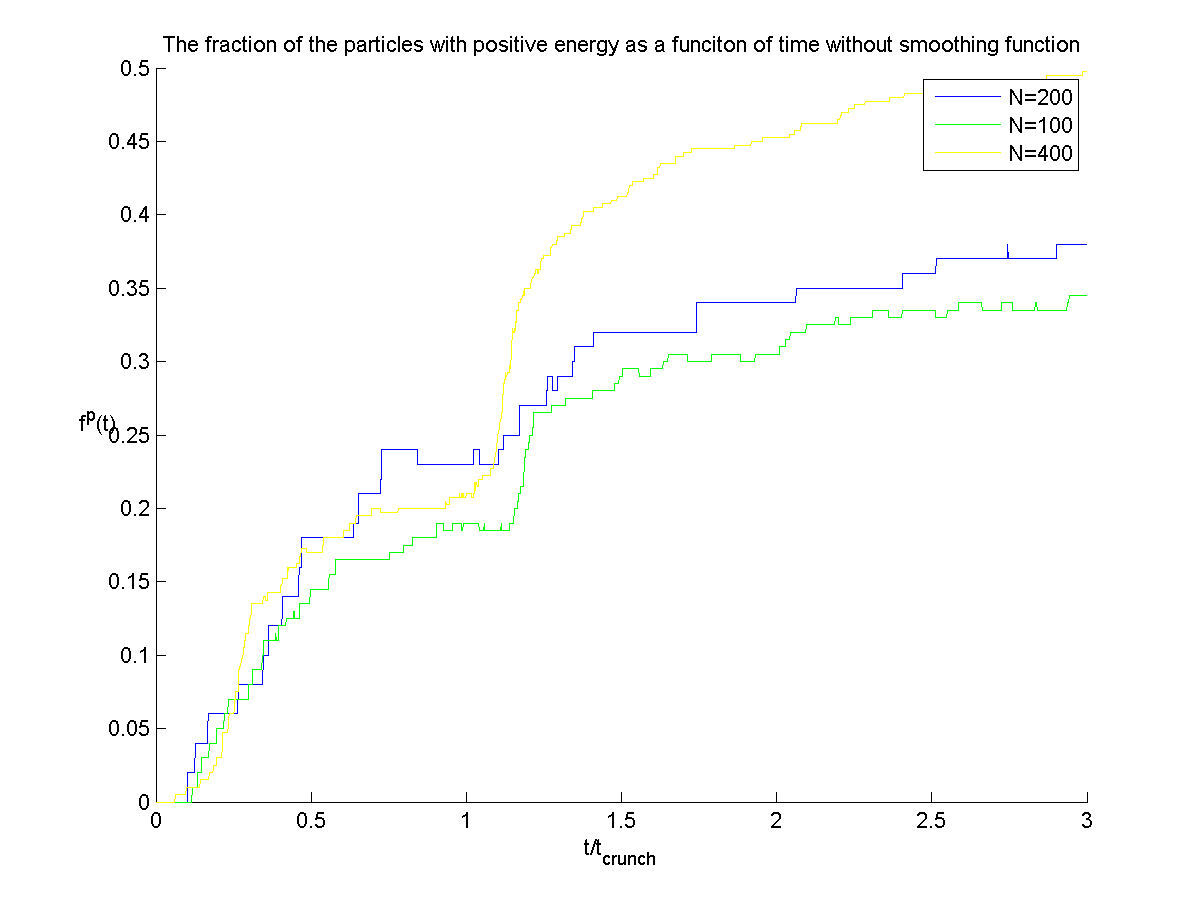
\includegraphics[width=0.8\textwidth]{d2.png}
\end{figure}
\begin{figure}[h]
	\caption{Energy of the system vs particles ejected for $N=100$, without smoothing function\label{d3}}
	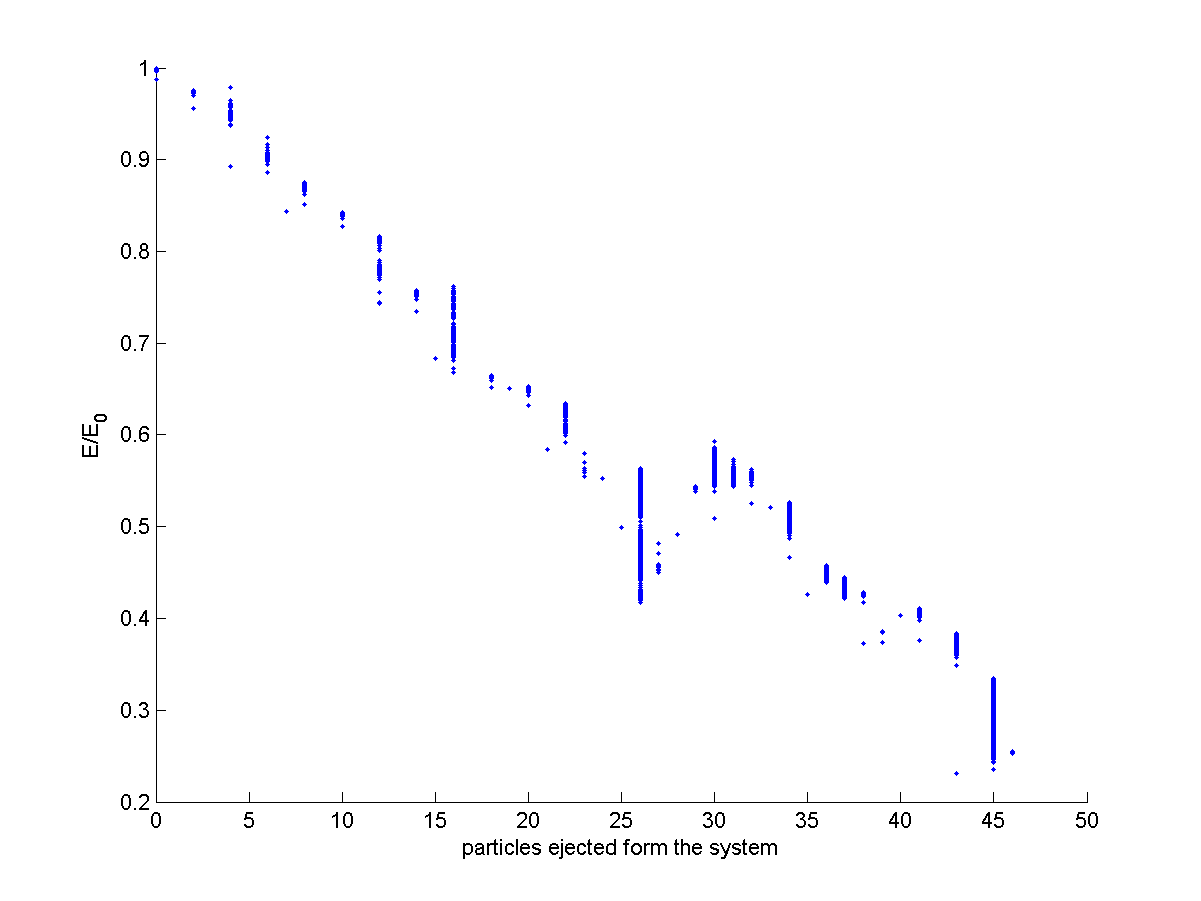
\includegraphics[width=0.8\textwidth]{d3.png}
\end{figure}


The previous results all show one important problem: We do not really conserve energy, as our system is not really realistic when it comes to small distances between two or more particles. Our objects are actually infinitely small mass points instead of bodies with a finite range like stars or planets! This can lead to serious problems. To demonstrate that, we can just take the case of a system with only $N=2$ particles starting at rest. In our model as well as in reality, those two particles would be accelerated towards each other and gain (negative) potential energy in the same way they gain (positive) kinetic energy; but in reality, those particles would, after some time, collide with each other. However, in our model, these particles will never collide as they have no extent! They can get closer and closer, leading to nearly infinitely high forces. In fact, they could even be at the exact same point in space which would imply an infinite force! Together with the finite, non-zero step length in time, these unrealistically high forces can lead to a velocity of the two stars that is high enough to make them unbound! To avoid this, it seems to be reasonable to introduce a smoothing function that guarantees finite forces even for small distances between the objects. This can be justified by the fact that in reality two extended objects cannot get infinitely close as described above. We set up this smoothing factor according to the project instructions by changing the pure Newtonian force in the following way:
\begin{equation}
F_\mathrm{mod}=-\frac{G*M_1*M_2}{r^2+\epsilon^2}
\end{equation}
where $\epsilon$ is a small real constant. We tried many different values of $\epsilon$, ending up with a value of $\epsilon=0.29$ giving us the best energy conservation. To show that, we plotted the total energy of our system again as function of time like we did in fig. \ref{d3}. The new plot in fig.\ref{e1} now looks completely different: We can see that for very short times, we can get high potential energy, but we never reach values lower than the initial energy. Although this diagram covers a time range more than ten times longer than in fig \ref{d3}, we have our energy conserved very well. This is one of the best tests we can implement for our algorithms as we do not have analytical solutions to the $N$-body problem that we can compare our results to! Even the very short peaks in the energy can be explained by our finite step length in time: It can happen that the planets get much closer to each other during one time step while still having the velocity that was calculated based on the force and acceleration of the previous step. As the velocity is somehow \glqq behind\grqq the force in time, we will often observe this behaviour where the potential increases before the velocity (and the kinetic energy) can settle accordingly. That means that we only have long term energy conservation while we can experience some short term peaks due to the finite step length. This long term conservation is delivered very well by our algorithm, justifying our choice of the smoothing factor.

\begin{figure}[h]
	\caption{The total energy of the system over time, with smoothing 		function\label{e1}}
	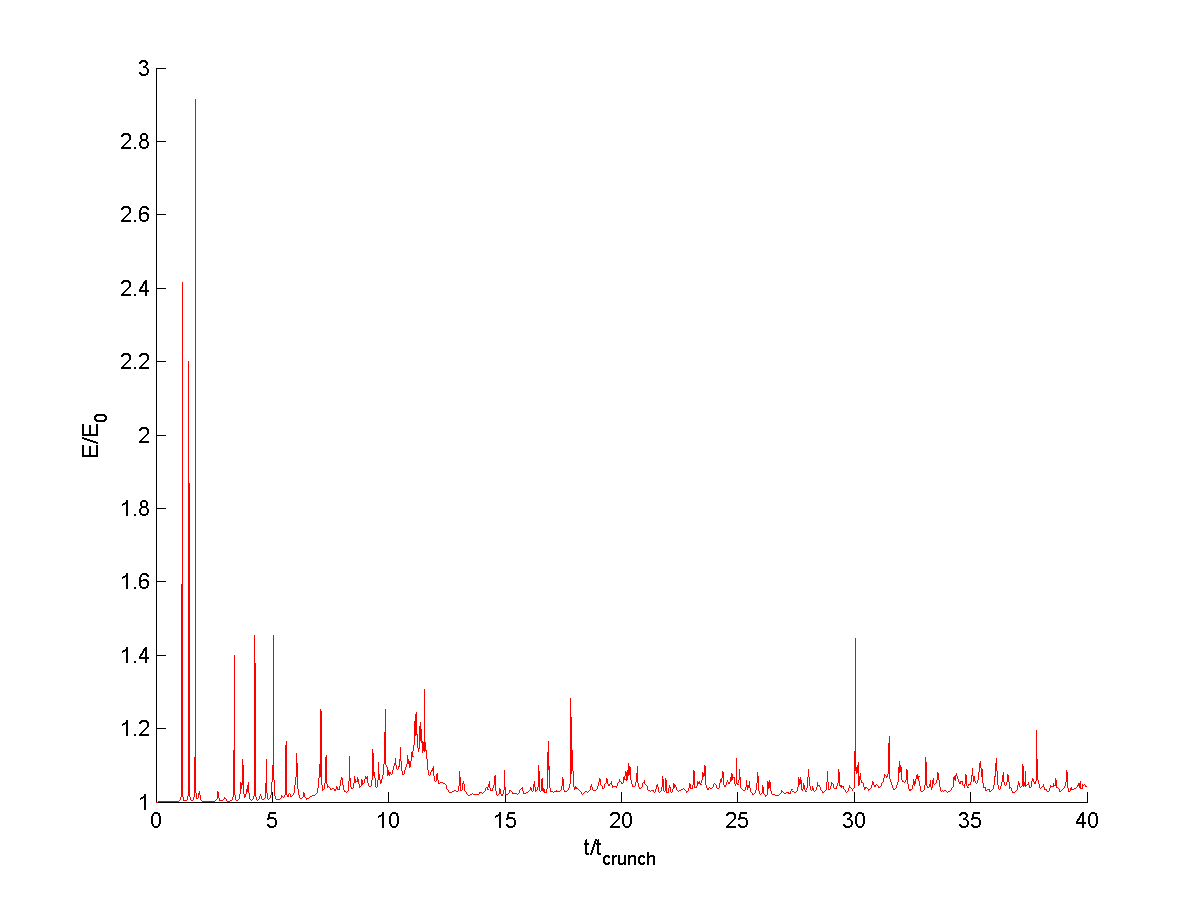
\includegraphics[width=0.8\textwidth]{e1.png}
\end{figure}

An interesting consequence of the newly introduced smoothing function can be seen in fig. \ref{e2}: This is basically the same plot as in fig. \ref{d2}, but now with this new factor. We can see that we now don't have any objects ejected until it comes to the first crunch! After that, many particles get ejected very fast in a way that is very similar to the behaviour that we experienced without smoothing function. Our system seems to be completely stable until it implodes for the first time.

\begin{figure}[h]
	\caption{The fraction of particles with positive energy (=ejected particles) as a function of time, with smoothing factor\label{e2}}
	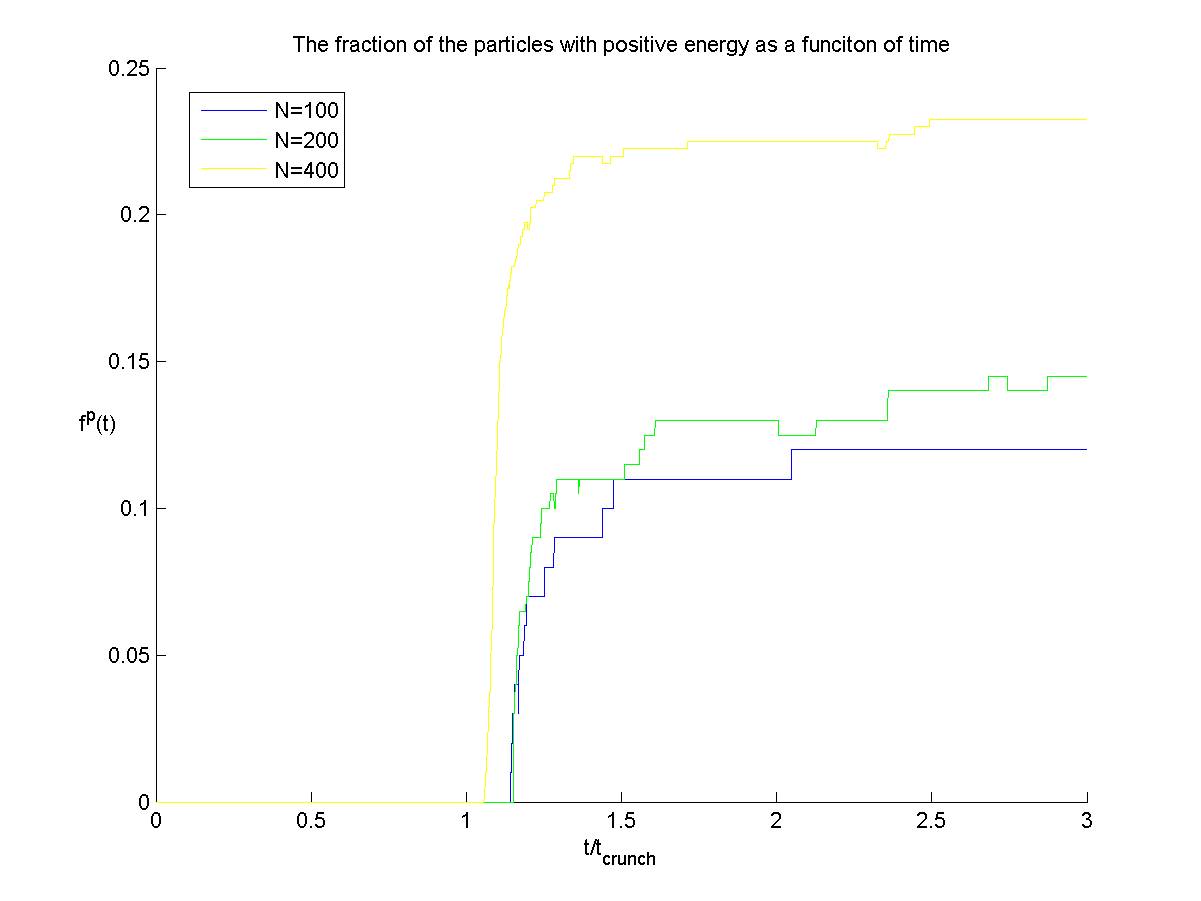
\includegraphics[width=0.8\textwidth]{e2.png}
\end{figure}

As mentioned before, there are not many test we can implement in our $N$-body system due to the lack of analytical solutions. We showed that our algorithm is consistent under the aspect of energy conservation and is able to reproduce a stable system until it crunches for the first time. But there is one more test that we can perform: We can check whether our program is able to validate the virial theorem. This theorem states the following equation for the averages over time of kinetic energy $<K>$ and potential energy $<V>$:
\begin{equation}
2<K>=-<V>
\end{equation}
We plotted the development of the ratio $<V>/<K>$ over time for one system in fig. \ref{f1}. We can clearly see that after a long time, we reach a stable state at $-2$. This is exactly the result that we expected through the virial theorem. This also underlines the exactness of the algorithm.

\begin{figure}[h]
	\caption{Energy of the system vs particles ejected for $N=100$, with smoothing function\label{f1}}
	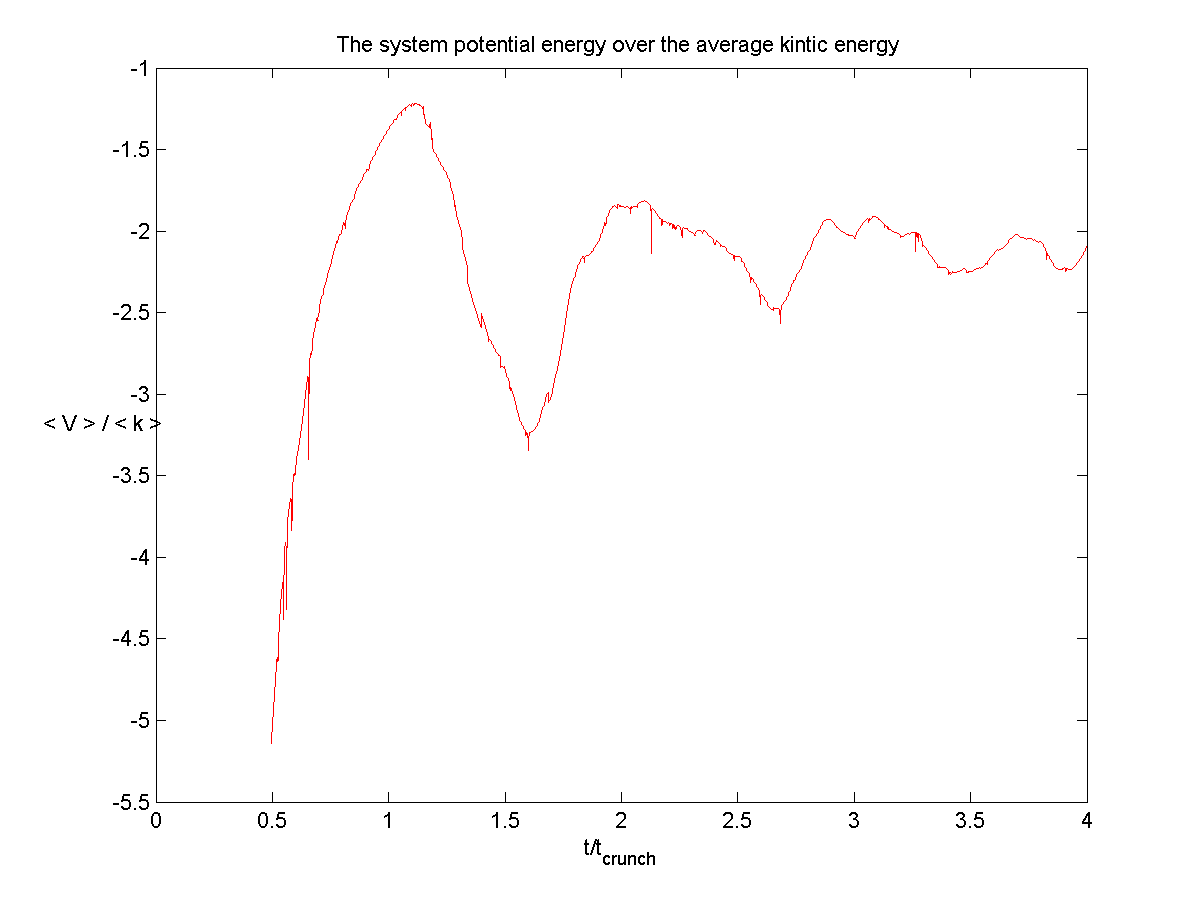
\includegraphics[width=0.8\textwidth]{f1.png}
\end{figure}

\section{Discussion}

\section{Source code}

\begin{thebibliography}{mustermarke}
\bibitem[1]{Link1} Source: \url{https://en.wikipedia.org/wiki/Open_cluster}, date: 10.12.2015 time: 17:00
\bibitem[2]{Link2} M. Joyce, B. Marcos, and F. Sylos Labini, Cold uniform spherical collapse revisited,
AIP Conf. Proc. 1241, 955 (2010);
\end{thebibliography}
\end{document}